\begin{figure}[H]
\centering
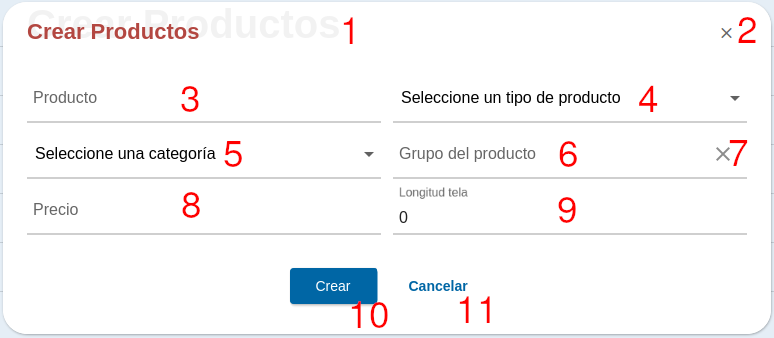
\includegraphics[width=\textwidth,height=\textheight,keepaspectratio]{Escenarios/AD-43-00}
\caption{Escenario - AD-43-00}
\label{fig:AD-43-00}
\end{figure}

Este escenario permite crear o modificar un producto, en \textbf{AD-43-01} se indicará la operación que se esté realizando mostrando 'Crear Productos' o 'Modificar Productos'. Con el botón \textbf{AD-43-02} se podrá volver al escenario \textbf{AD-42-00}. Se debe ingresar un nombre de producto en \textbf{AD-43-03}, la lista desplegable \textbf{AD-43-04} permite indicar un tipo de producto, la lista desplegable \textbf{AD-43-04} permite indicar una categoría de producto, el usuario además debe indicar el grupo de producto en el campo \textbf{AD-43-06}, el cual cuenta con el botón \textbf{AD-43-07} para borrar el texto ingresado en el campo, también debe ingresar un precio en \textbf{AD-43-08} y la longitud de tela en \textbf{AD-43-09}. En caso de estar modificando un producto, los campos \textbf{AD-43-03}, \textbf{AD-43-04}, \textbf{AD-43-05}, \textbf{AD-43-06}, \textbf{AD-43-08} y \textbf{AD-43-09} estarán autocompletados con los valores actuales del producto, pudiendo modificar los mismos. Al hacer click en el botón \textbf{AD-43-10} se modificará o creará el producto según corresponda, mostrando en el botón el texto 'Crear' o 'Modificar' respectivamente. Con el botón \textbf{AD-43-11} se podrá volver al escenario \textbf{AD-42-00} cancelando la operación que se esté realizando.
\clearpage
